\documentclass{article}
\usepackage[
paperwidth = 14cm, 
textwidth = 14cm,
paperheight=8cm, 
textheight =8cm,
nohead,
nofoot,
nomarginpar,
margin=0mm]{geometry}
\usepackage{amsmath,amsfonts,amssymb}
\usepackage{tikz,pgfplots}
\usetikzlibrary{arrows,arrows.meta,bending,calc,decorations,shadings,shadows,shapes,shapes.arrows,shapes.geometric}
\usetikzlibrary{calc,fadings,decorations.pathreplacing}
\usepgfplotslibrary{units,fillbetween,groupplots,colorbrewer}
\usetikzlibrary{pgfplots.colorbrewer,}
\usepackage{pgfplotstable}
\usetikzlibrary{3d,spy}
\usepgfmodule{plot}
\usepackage{scalerel}
\usepackage{graphicx}
\usepackage{tikz-dimline}
\usepackage{epstopdf}
\epstopdfsetup{outdir=out/,suffix=-generated}
\definecolor{As}{RGB}{255,255,0}
\definecolor{Al}{RGB}{173,216,230}
\definecolor{Ga}{RGB}{0,128,150}

%\definecolor{background}{RGB}{77,77,77}
\definecolor{background}{RGB}{255,255,255}

\definecolor{plane100}{RGB}{0,178,69}
\definecolor{plane010}{RGB}{0,255,208}

\newcommand*{\xMin}{0}%
\newcommand*{\xMax}{14}%
\newcommand*{\yMin}{-7}%
\newcommand*{\yMax}{0}%

\begin{document}
	\thispagestyle{empty}
\begin{tikzpicture}[remember picture,overlay]
% \draw[fill=background] (current page.north west)--
% 	(current page.south west)--
% 	(current page.south east)-- 
% 	(current page.north east) --cycle;

% \foreach \i in {\xMin,...,\xMax} {
% 	\draw [very thin,gray] (\i,\yMin) -- (\i,\yMax)  node [below] at (\i,\yMin) {$\i$};
% }
% \foreach \i in {\yMin,...,\yMax} {
% 	\draw [very thin,gray] (\xMin,\i) -- (\xMax,\i) node [left] at (\xMin,\i) {$\i$};
% }

	
\node[anchor=south,inner sep=0mm,yshift=0mm,xscale=-1](s1) at (current page.south)
	{
	\includegraphics[width=\textwidth,trim={0cm 0cm 0 0cm},clip]{/media/labfiles/ruco/phd-ssp/phd-codes/symmetry/acqws-symmetry1-out.pdf}
	};

\begin{scope}[yshift=-24mm]

\def\amp{0.5mm}
\def\len{7mm}

\def\yi{-1.9}
\def\yf{-5.1}

\draw[fill=Al,fill opacity=0.0,draw=Al,line width=0.5mm](-0.3,\yf)--(3.6,\yf) decorate [decoration={snake,segment length=\len,amplitude=\amp}]{--(3.6,\yi)} --(0,\yi) decorate [decoration={snake,segment length=\len,amplitude=\amp}]{--(0,\yf)};


\draw[fill=Ga,fill opacity=0.0,draw=Ga,line width=0.5mm](4.0,\yf)--(4.8,\yf) decorate [decoration={snake,segment length=\len,amplitude=\amp}]{--(4.8,\yi)} --(4.0,\yi) decorate [decoration={snake,segment length=\len,amplitude=\amp}]{--(4.0,\yf)};


\draw[fill=Al,fill opacity=0.0,draw=Al,line width=0.5mm](5.2,\yf)--(6.0,\yf) decorate [decoration={snake,segment length=\len,amplitude=\amp}]{--(6.0,\yi)} --(5.2,\yi) decorate [decoration={snake,segment length=\len,amplitude=\amp}]{--(5.2,\yf)};


\draw[fill=Ga,fill opacity=0.,draw=Ga,line width=0.5mm](6.3,\yf)--(9,\yf) decorate [decoration={snake,segment length=\len,amplitude=\amp}]{--(9,\yi)} --(6.3,\yi) decorate [decoration={snake,segment length=\len,amplitude=\amp}]{--(6.3,\yf)};

\draw[fill=Al,fill opacity=0.0,draw=Al,line width=0.5mm](9.3,\yf)--(13,\yf) decorate [decoration={snake,segment length=\len,amplitude=\amp}]{--(13,\yi)} --(9.3,\yi) decorate [decoration={snake,segment length=\len,amplitude=\amp}]{--(9.3,\yf)};
\end{scope}


\begin{scope}[yshift=0cm,rotate around y=180,xshift=12.8cm]
	\draw[black,densely dashed](0,0)--++(3.8,0)--++(0,-2)--++
	(3,0)--++(0,2)--++(1.0,0)--++(0,-2)--++(1.2,0)--++(0,2)--++(4,0);
	
	\draw[black, densely dashed] (0,-4)--++(3.8,0)--++(0,1)--++
	(3,0)--++(0,-1)--++(1.0,0)--++(0,1)--++(1.2,0)--++(0,-1)--++(4,0);

\node[xshift=0mm,yshift=0mm](a1) at (3.8,-1){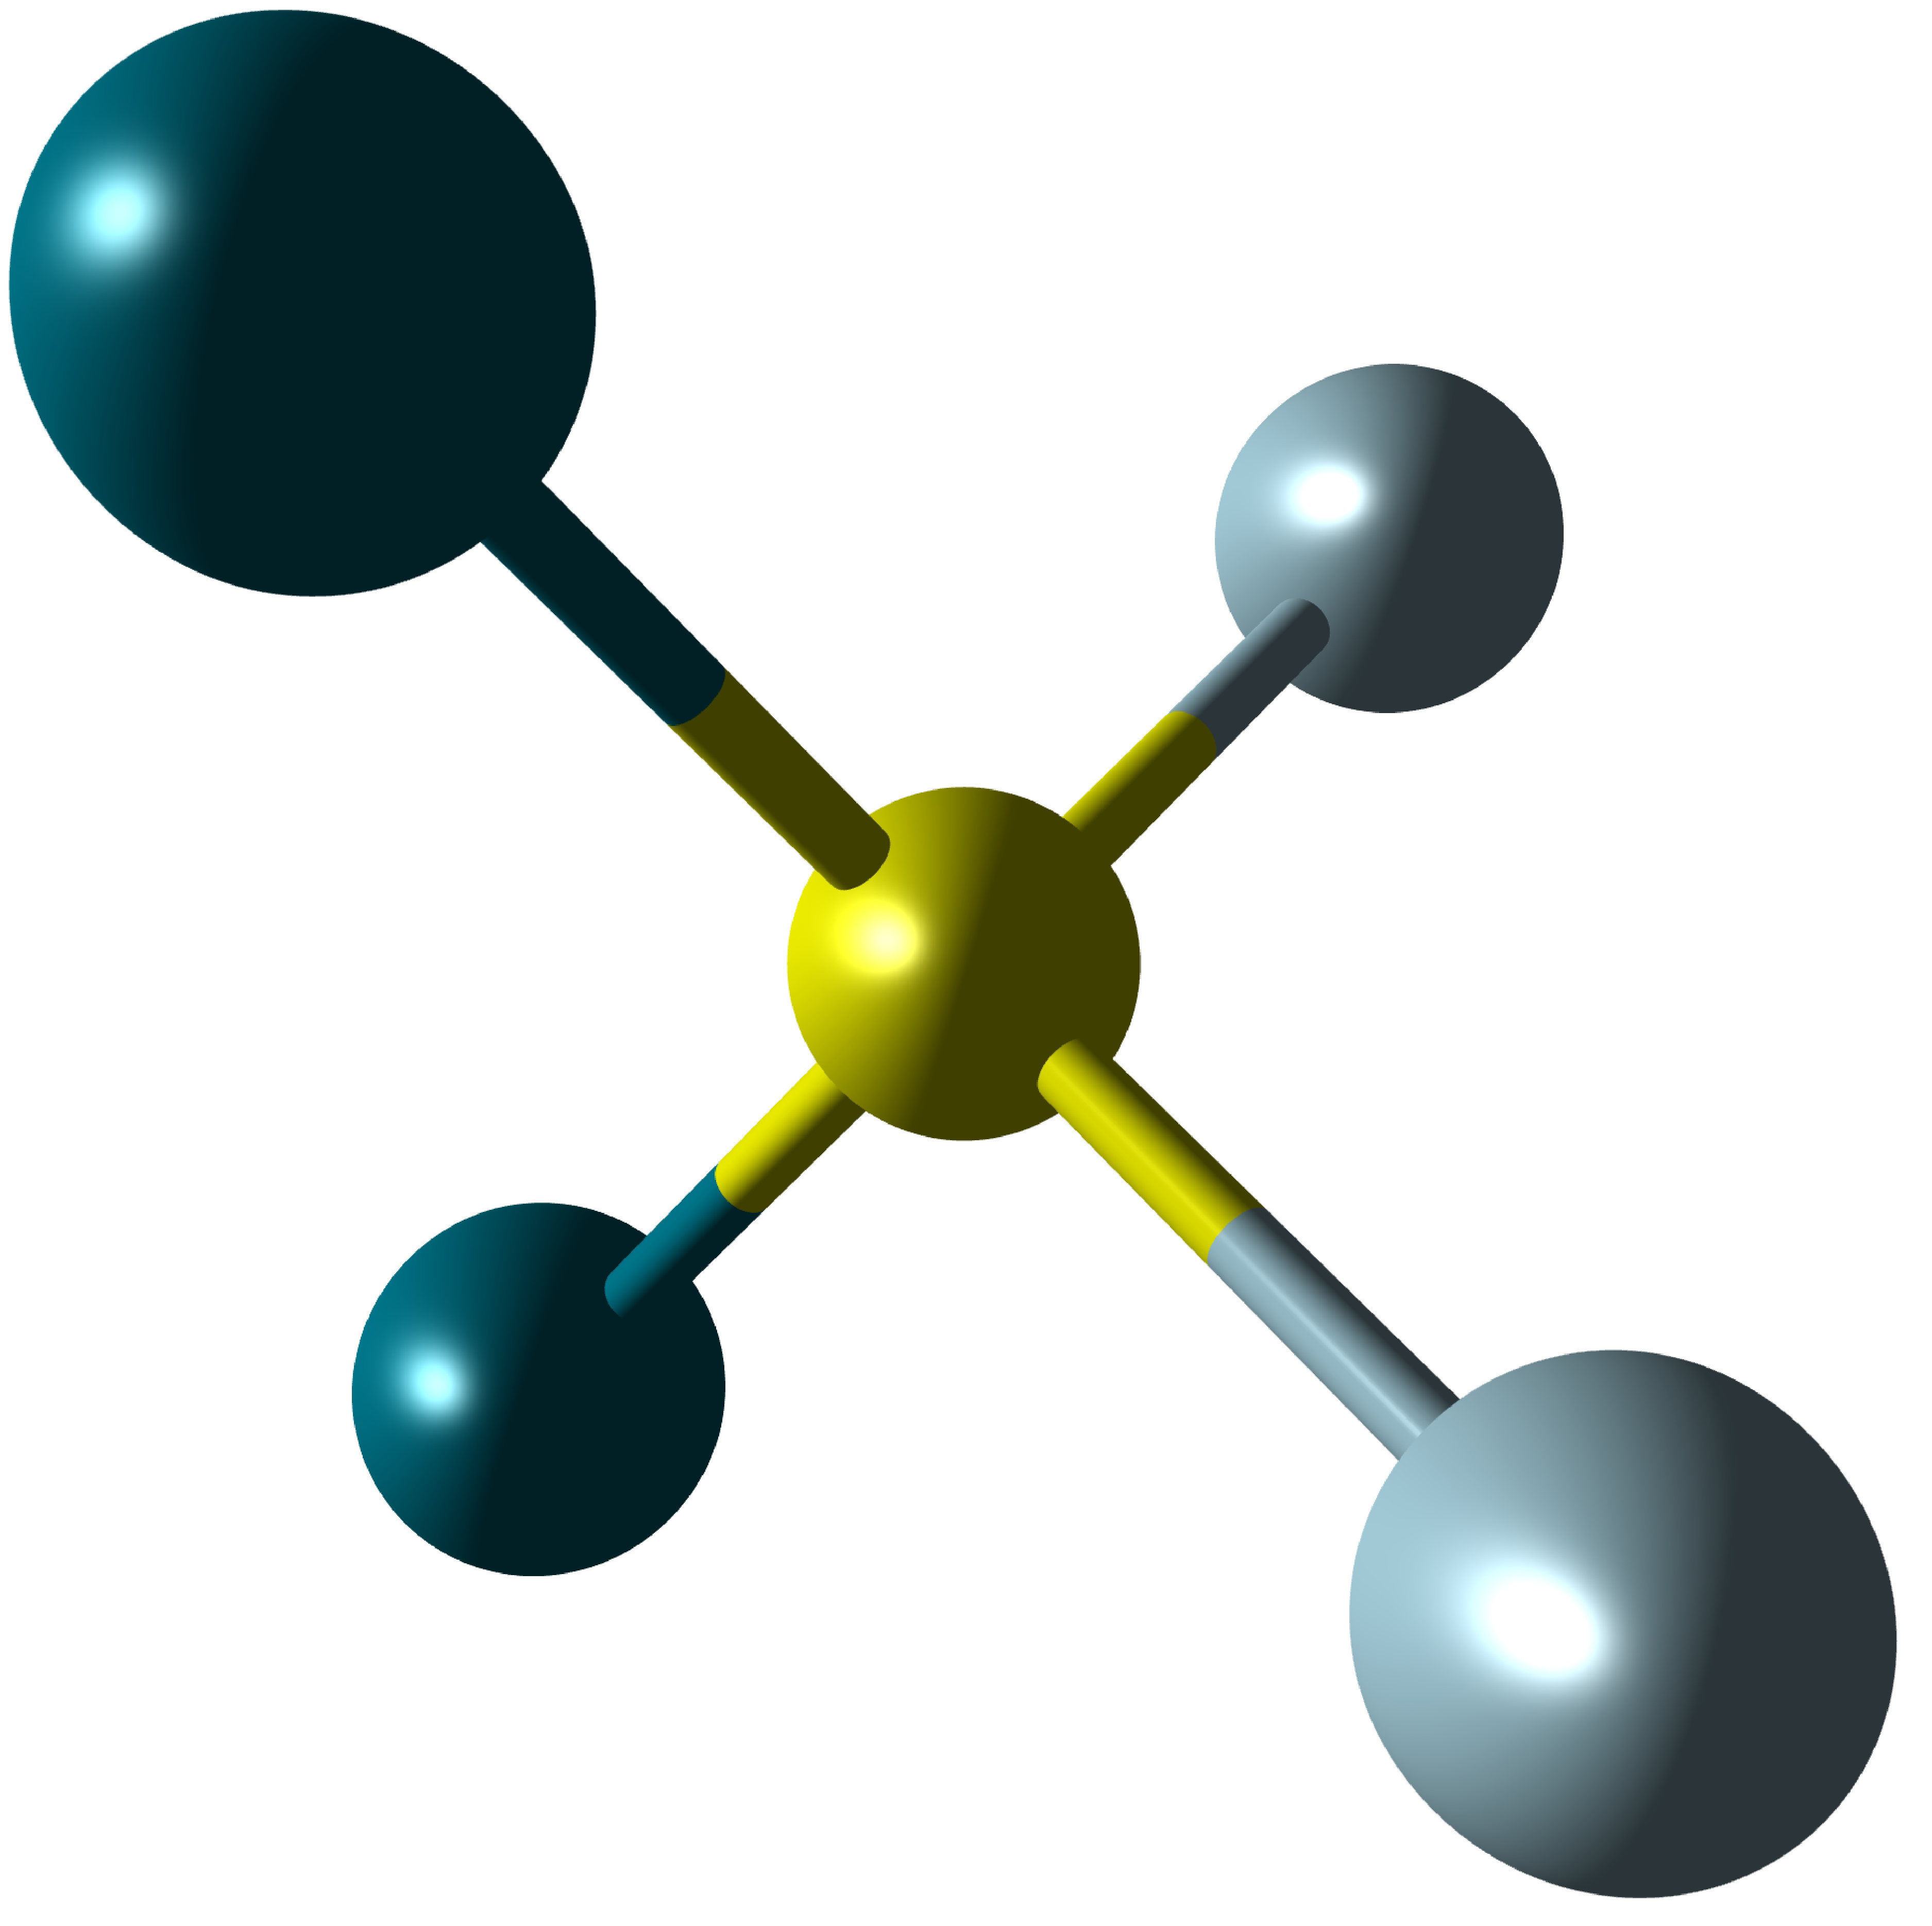
\includegraphics[width=0.09\textwidth]{/media/labfiles/ruco/phd-ssp/phd-codes/symmetry/algaas-interface-1-out.pdf}};

\node[anchor = center,xshift=0mm,yshift=0mm](a2) at (3.8+3,-1){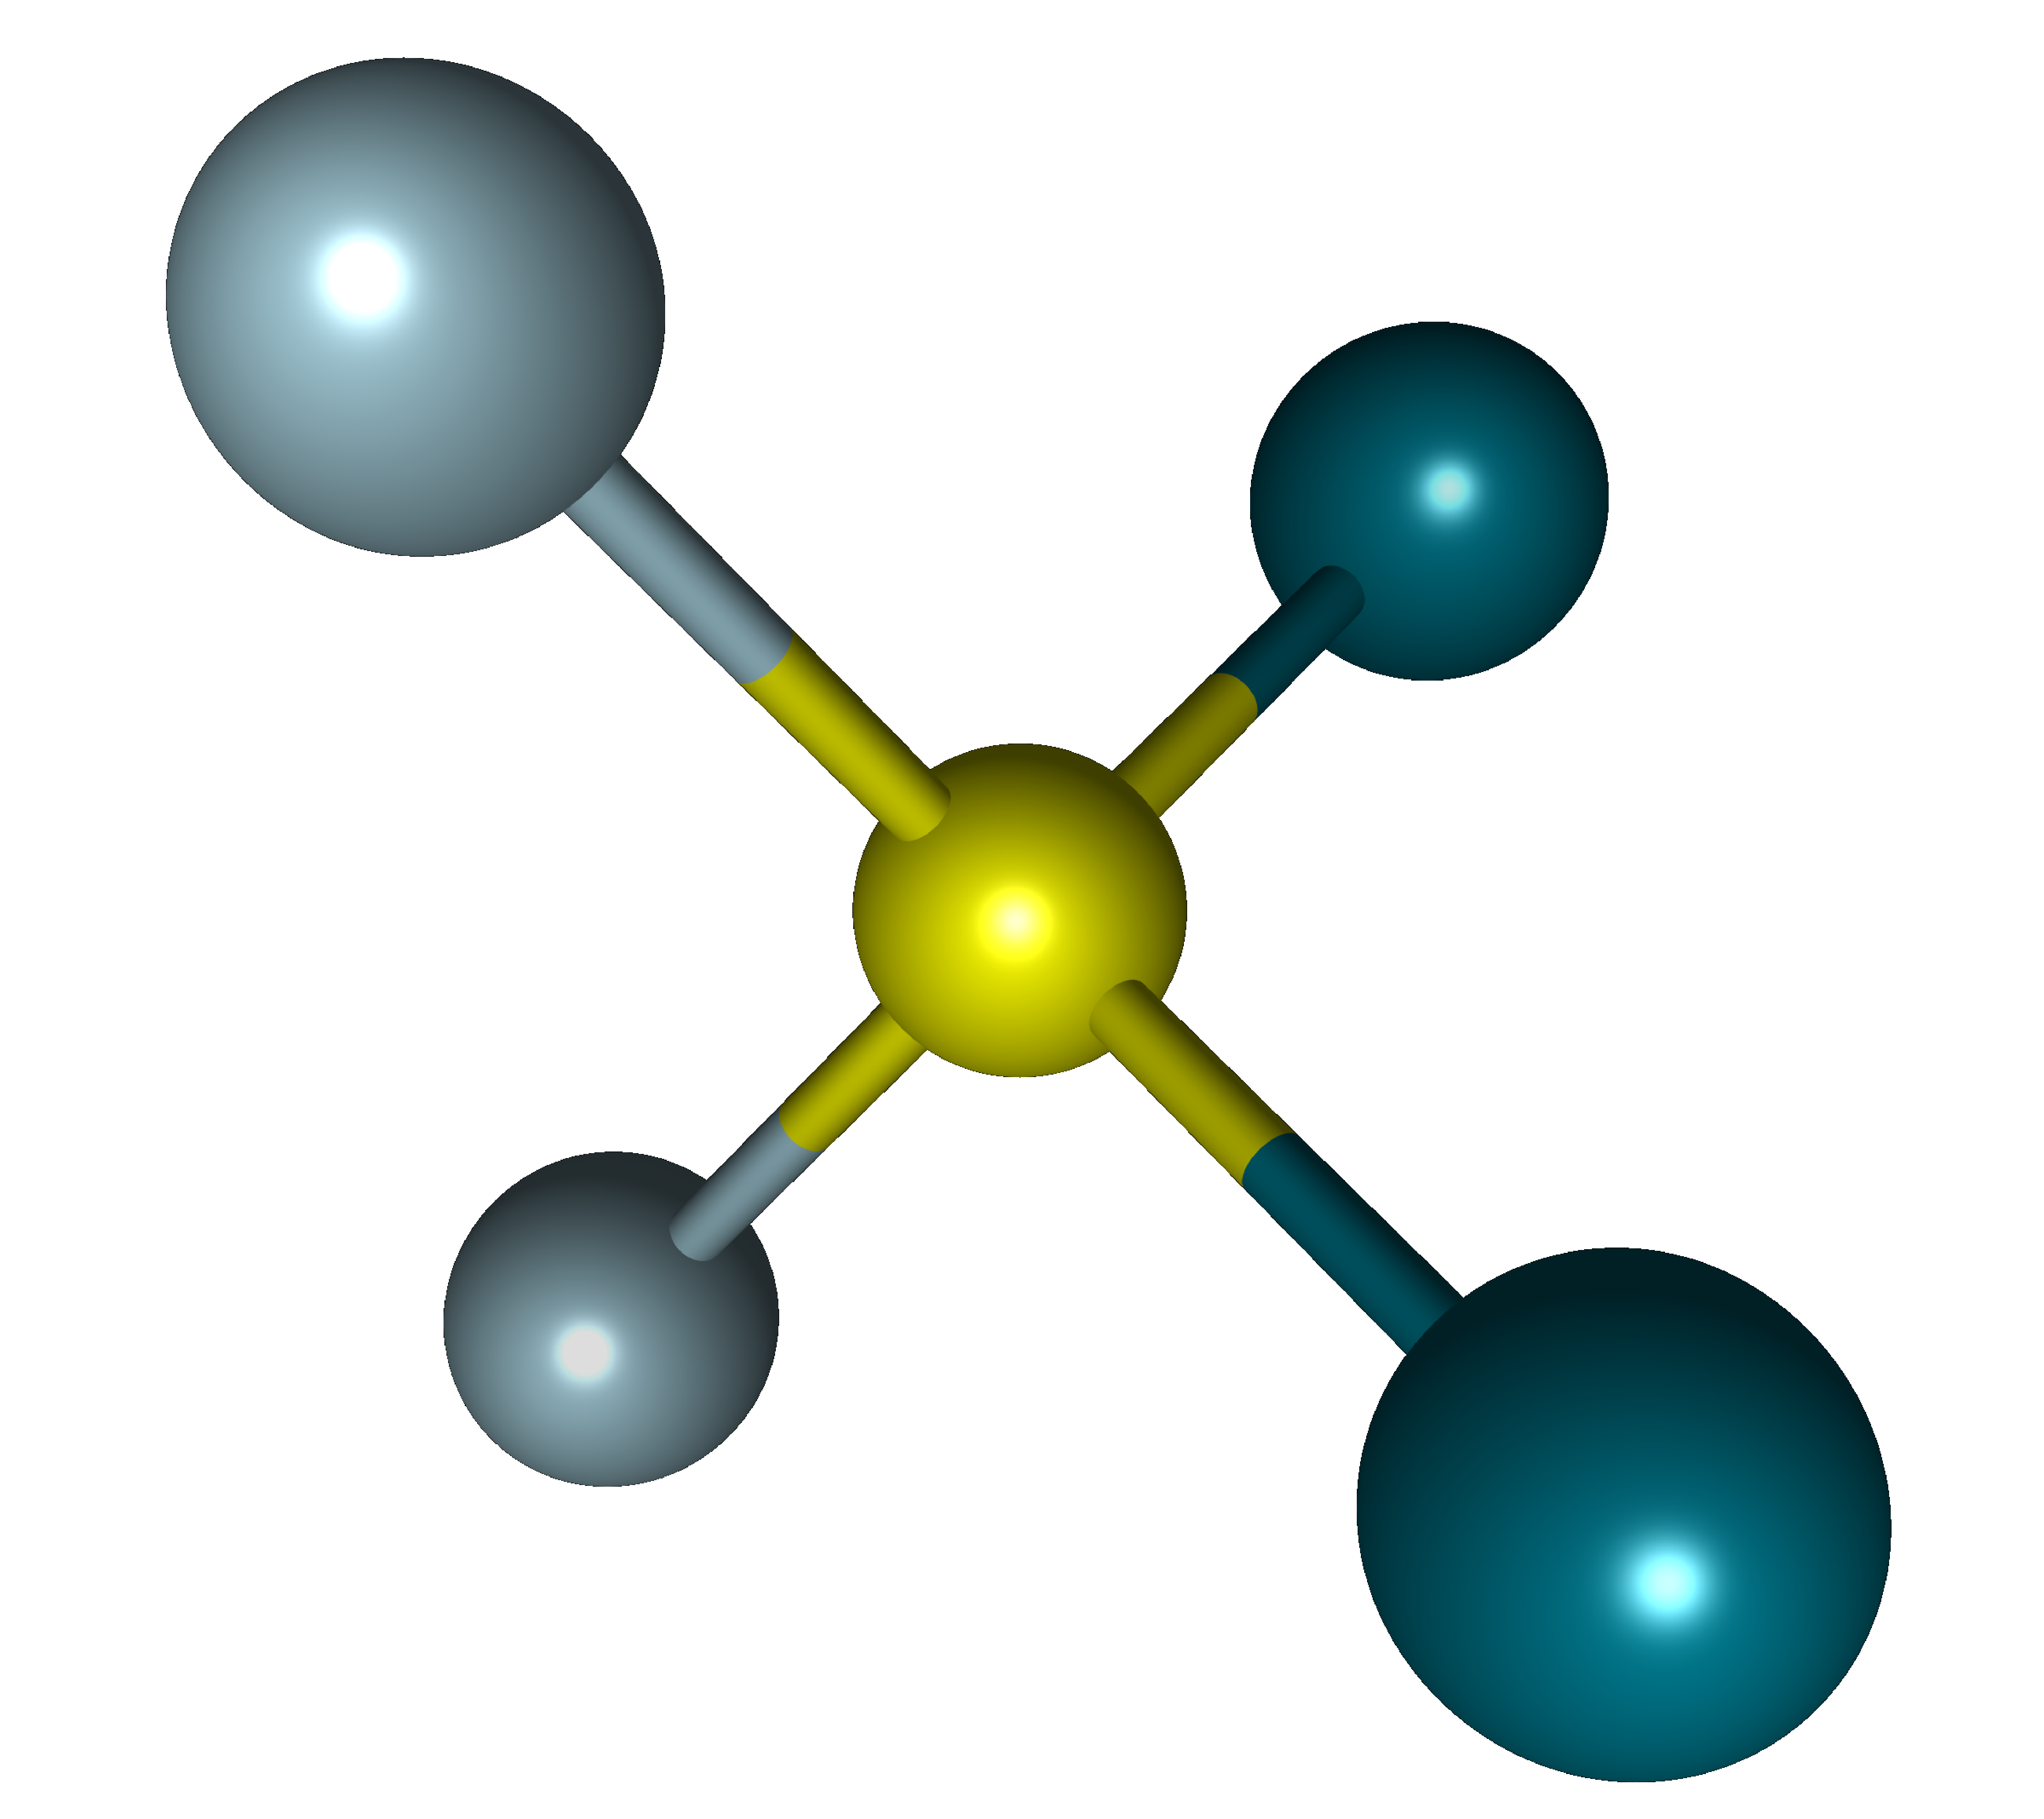
\includegraphics[width=0.09\textwidth]{/media/labfiles/ruco/phd-ssp/phd-codes/symmetry/algaas-interface-0-out.pdf}};

\node[anchor=center,xshift=0mm,yshift=0mm](a3) at (3.8+3+1,-1){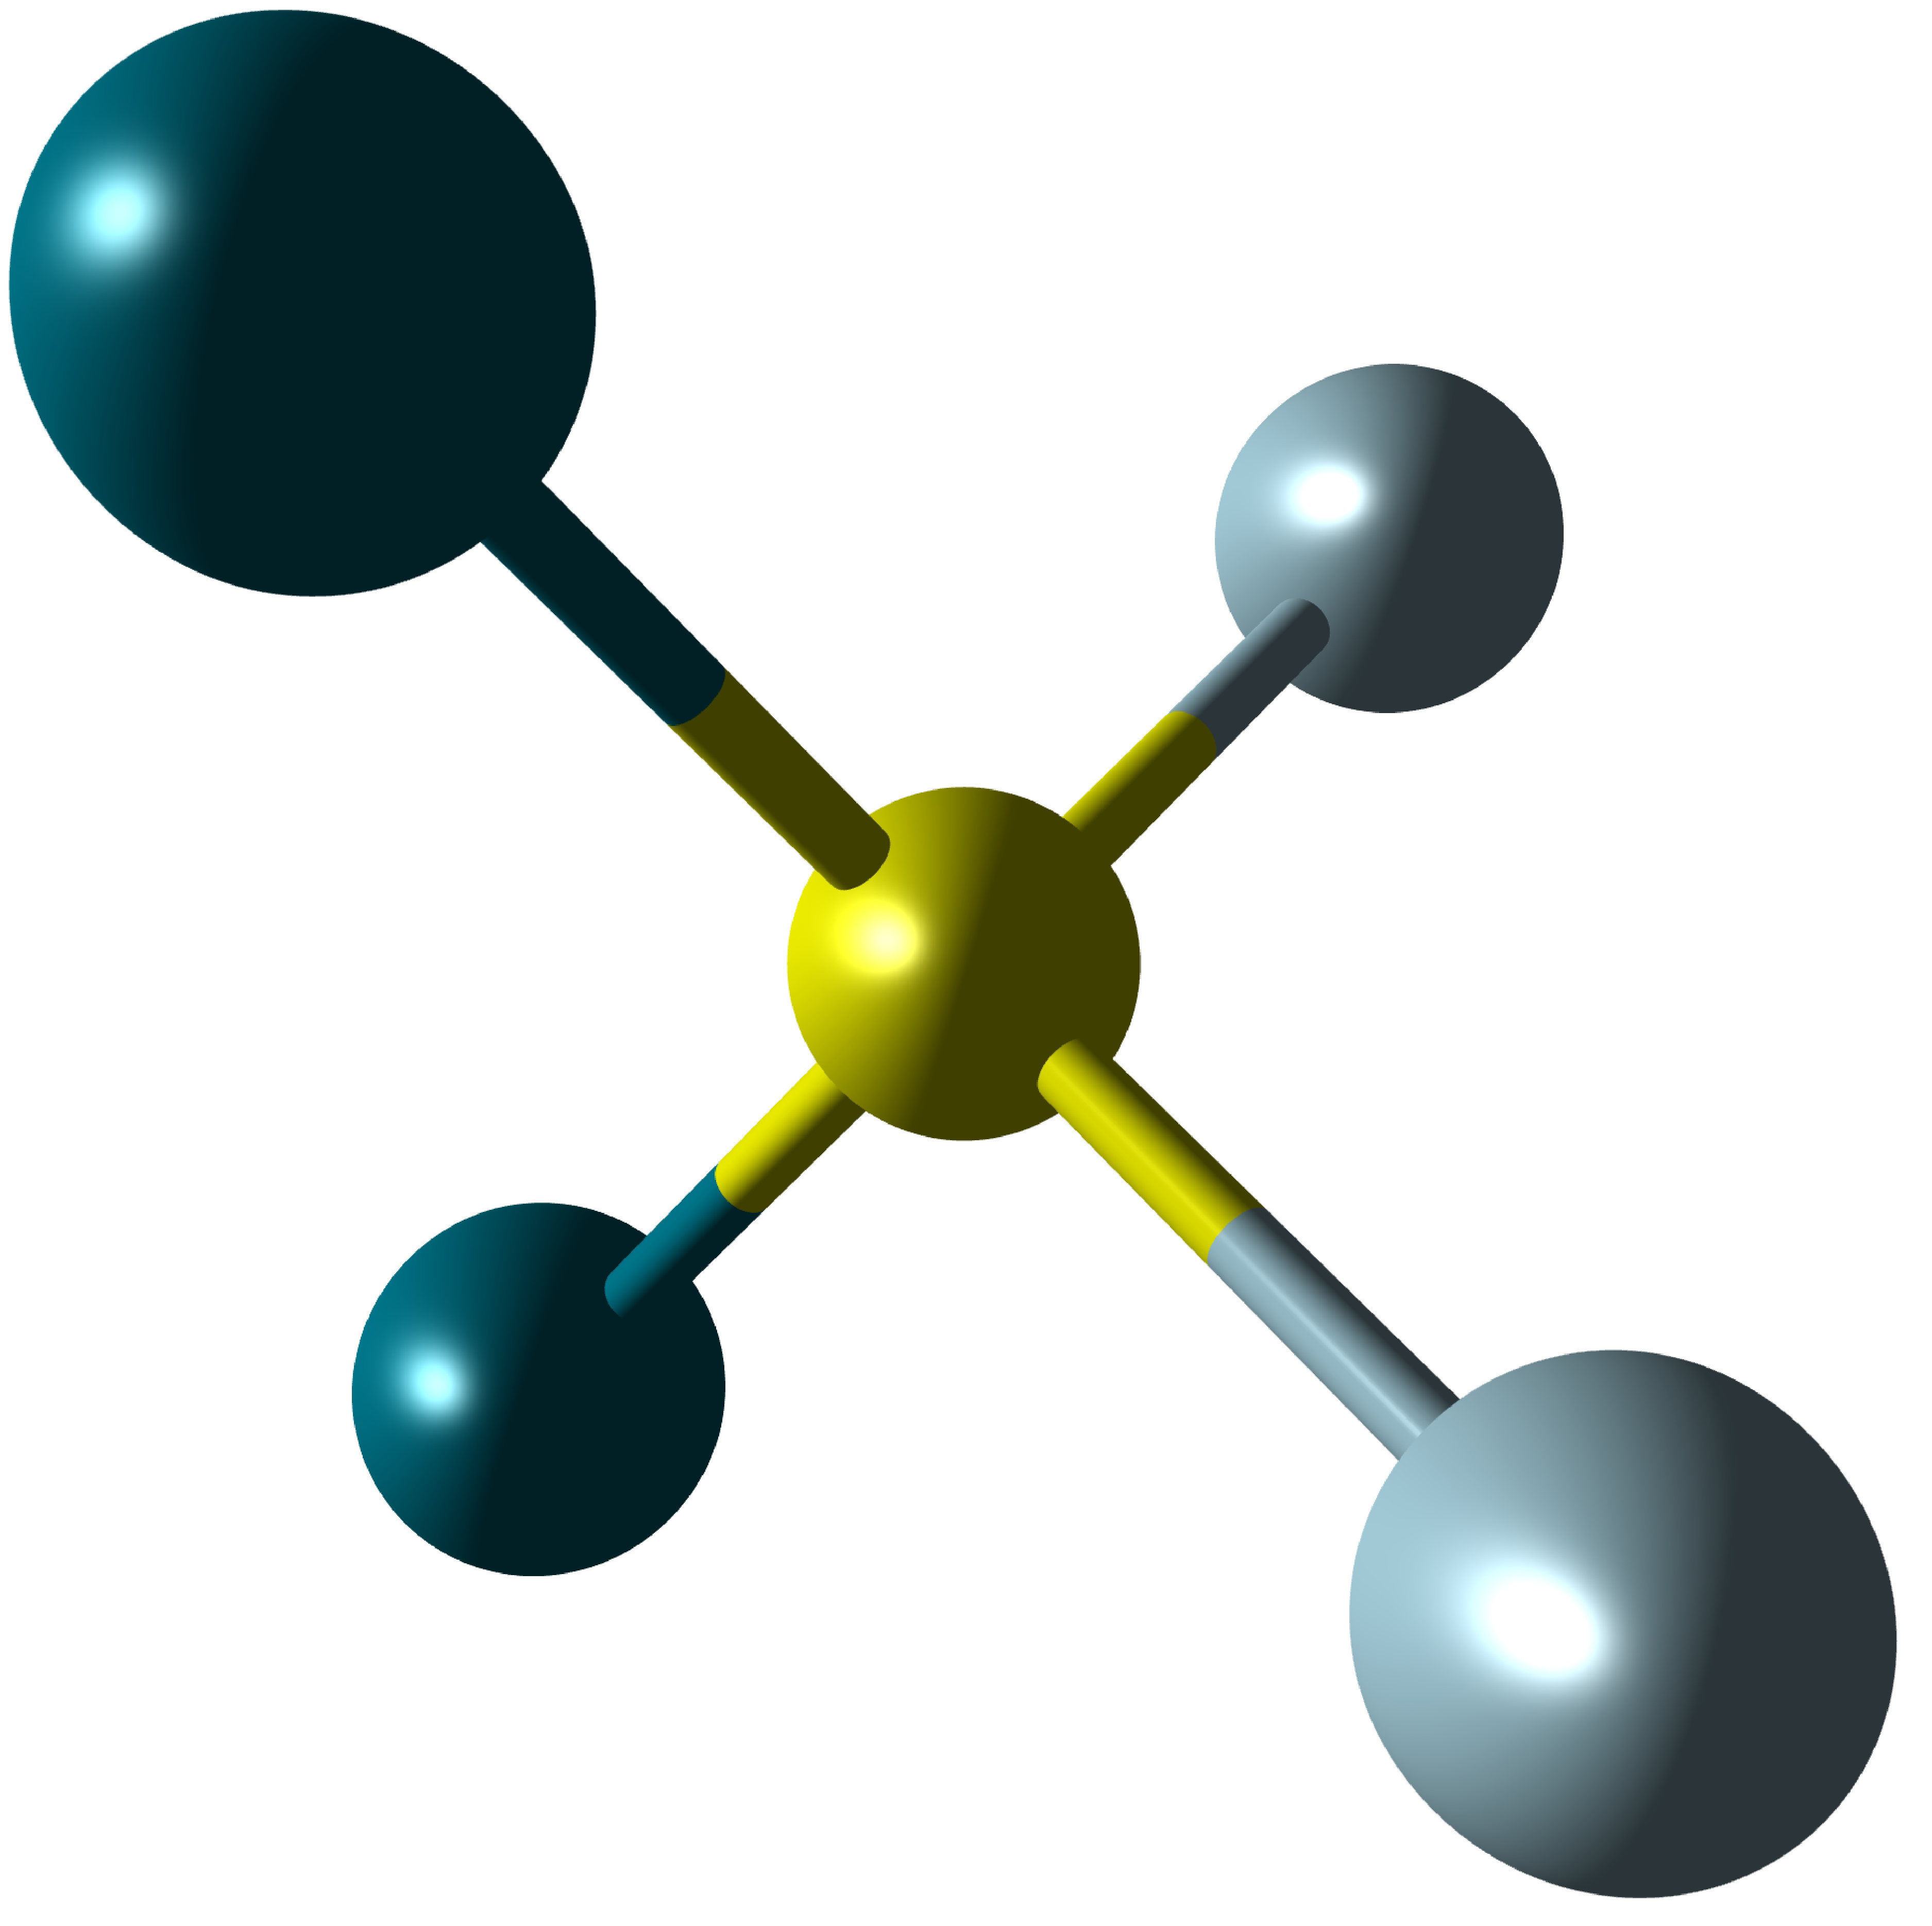
\includegraphics[width=0.09\textwidth]{/media/labfiles/ruco/phd-ssp/phd-codes/symmetry/algaas-interface-1-out.pdf}};

\node[anchor = center,xshift=0mm,yshift=0mm](a4) at (3.8+3+1+1.2,-1){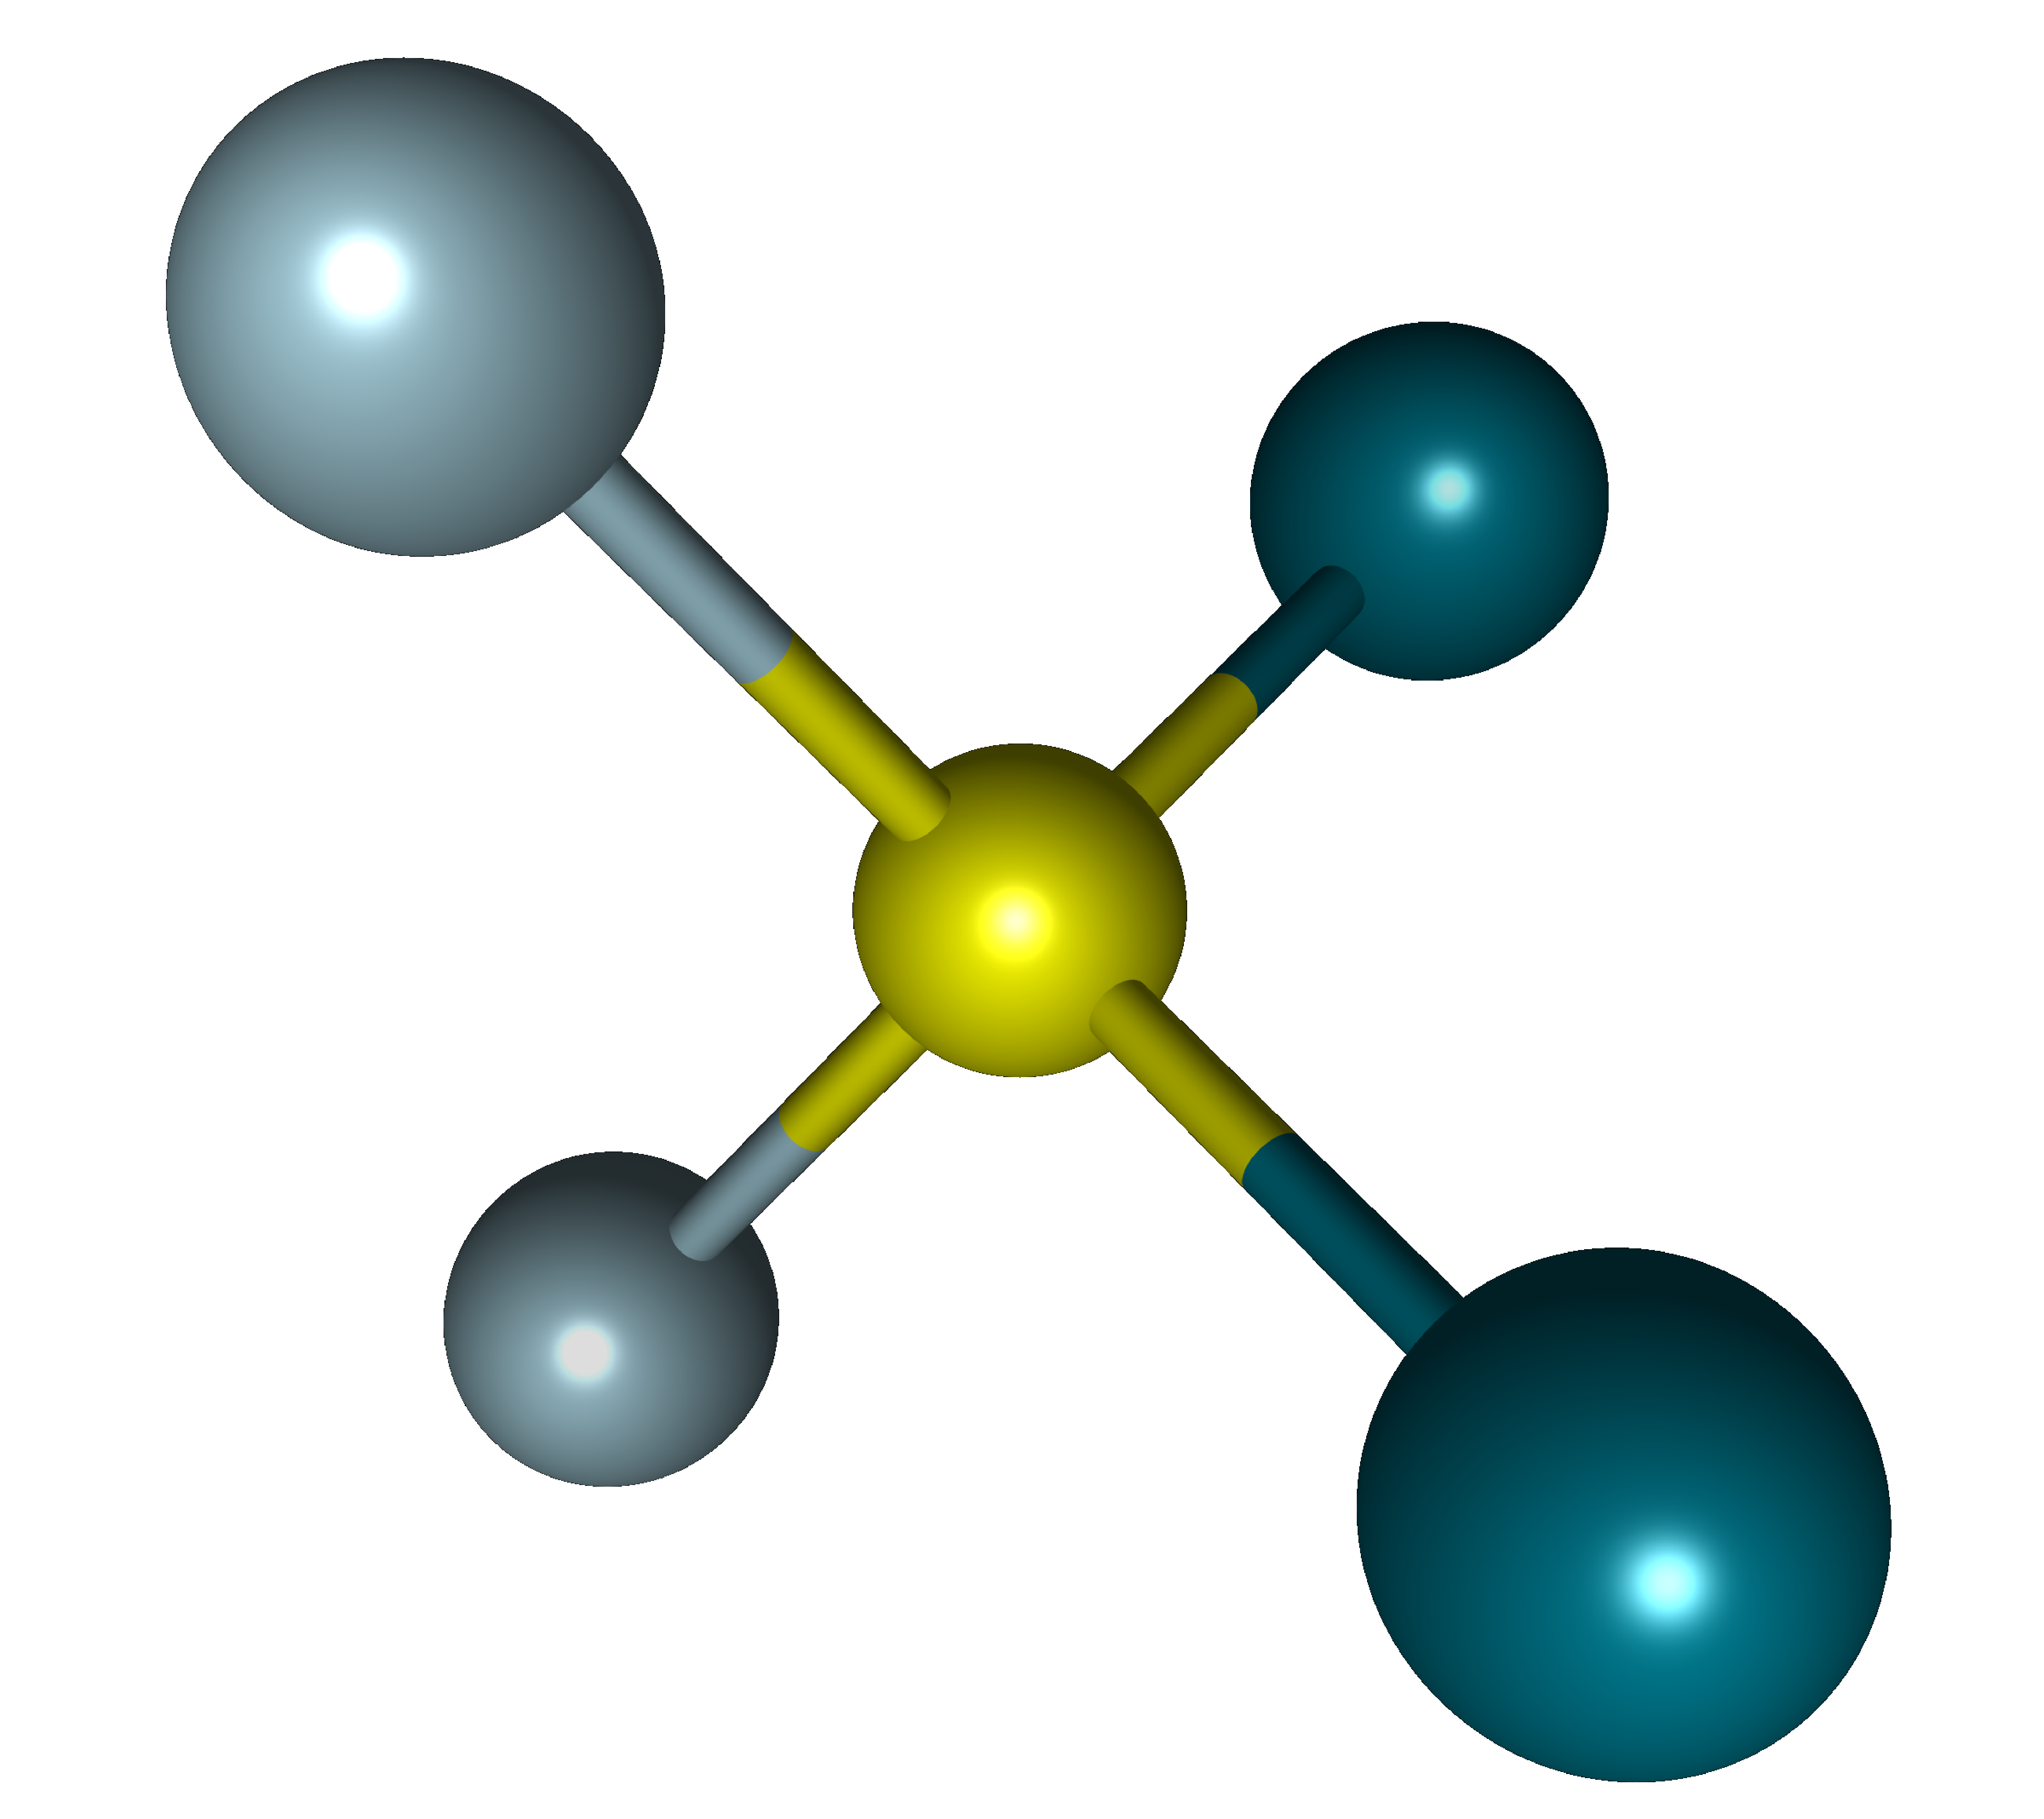
\includegraphics[width=0.09\textwidth]{/media/labfiles/ruco/phd-ssp/phd-codes/symmetry/algaas-interface-0-out.pdf}};
\end{scope}


\begin{scope}[xshift=1cm,yshift=-2.7cm,rotate around y=-10,scale=1.25]
	\draw[very thick,-{Stealth},green] (0,0,0) -- (0,0,1.9) node[anchor=south,yshift=2mm,scale=1.5]{$x$};
	\draw[very thick,-{Stealth},red]   (0,0,0) -- (0,1.9,0) node[anchor=west,yshift=-2mm,scale=1.5]{$y$};
	\draw[very thick,-{Stealth},blue]  (0,0,0) -- (1.9,0,0) node[anchor=west,scale=1.5]{$z$};
	\draw[fill=gray,fill opacity=0.2,draw=black,line width=0.05mm] (0,0,0)--(1.5,0,0)--(1.5,1.5,0)--(0,1.5,0)--cycle;
	\draw[fill=gray,fill opacity=0.2,draw=black,line width=0.05mm] (0,0,0)--(0,1.5,0)--(0,1.5,1.5)--(0,0,1.5)--cycle;
	\draw[fill=gray,fill opacity=0.2,draw=black,line width=0.05mm] (0,0,0)--(0,0,1.5)--(1.5,0,1.5)--(1.5,0,0)--cycle;

\def\textplanecolor{black}
	\node[canvas is yz plane at x = 0,rotate=270,scale=1.2,font=\boldmath,\textplanecolor] at (0,0.75,0.7) 
	 {$z_{_{\parallel}}(001)$};
	\node[canvas is zx plane at y = 0,rotate=90,scale=1.2,font=\boldmath,\textplanecolor] at (0.75,0,0.75) 
	 {$x_{_{\parallel}}(100)$};
	 \node[canvas is xy plane at z = 0,rotate=0,scale=1.2,font=\boldmath,\textplanecolor] at (0.75,0.75,0) 
	 {$y_{_{\parallel}}(010)$};
\end{scope}



\node[anchor=north east,fill=blue,text=white,inner sep=0mm,scale=1.5,font=\bfseries] (l1) at (current page.north east){(a)};

\node[anchor=south east, fill=blue,text=white,inner sep=0mm,scale=1.5,font=\bfseries] (l1) at (current page.south east){(b)};




\dimline[color=black,
	label style={fill=background,scale=1.2},
	line style={arrows=Stealth-Stealth,line width=0.2mm},
	extension start length=-0.2,
	extension end length=-0.2] {(3.8,-2.4)}{(3.8+1.2,-2.4)}{$d_{1}$};

\dimline[color=black,
	label style={fill=background,scale=1.2},
	line style={arrows=Stealth-Stealth,line width=0.2mm},
	extension start length=-0.2,
	extension end length=-0.2] {(3.8+1.2+1,-2.4)}{(3.8+3+1+1.2,-2.4)}{$d_{2}$};


\end{tikzpicture}
	
	


\end{document}